% $Header: /cvsroot/latex-beamer/latex-beamer/solutions/generic-talks/generic-ornate-15min-45min.en.tex,v 1.5 2007/01/28 20:48:23 tantau Exp $

\documentclass{beamer}
%\usecolortheme[RGB={205,173,0}]{structure} %Gold
\usecolortheme[RGB={218, 165, 32}]{structure} %Golden Rod
% This file is a solution template for:

% - Giving a talk on some subject.
% - The talk is between 15min and 45min long.
% - Style is ornate.
\usepackage{epstopdf} %put by hand to use .eps files with pdflatex
%\usepackage{longtable}
\usepackage{multirow}

% Copyright 2004 by Till Tantau <tantau@users.sourceforge.net>.
%
% In principle, this file can be redistributed and/or modified under
% the terms of the GNU Public License, version 2.
%
% However, this file is supposed to be a template to be modified
% for your own needs. For this reason, if you use this file as a
% template and not specifically distribute it as part of a another
% package/program, I grant the extra permission to freely copy and
% modify this file as you see fit and even to delete this copyright
% notice. 


\mode<presentation>
{
  %\usetheme{Singapore}
  \usetheme{Madrid}
  % or ...

  \setbeamercovered{transparent}
  % or whatever (possibly just delete it)
}


\usepackage[english]{babel}
% or whatever

\usepackage[latin1]{inputenc}
% or whatever

\usepackage{times}
\usepackage[T1]{fontenc}

\title[3D Pixels] % (optional, use only with long paper titles)
{My Contribution to the Testing and Characterization of the CMS Prototype 3D Silicon Pixel Detectors}

%\subtitle
%{Status Update} % (optional)
\author[Matthew Kress] % (optional, use only with lots of authors)
{Matthew Kress}
% - Use the \inst{?} command only if the authors have different
%   affiliation.

\institute[Purdue University] % (optional, but mostly needed)


\date[Friday Nov 1, 2013] % (optional)
{Friday Nov 1, 2013}

\subject{Talks}



\begin{document}

\begin{frame}
  \titlepage
\end{frame}


\begin{frame}{Introduction}
  \begin{center}
    This presentation is to go over my contribution to the characterization and test results of the 3D silicon CMS Pixel detectors at Purdue University.
    %\begin{itemize}
    %\item
    %\item
    %\item
    %\item
    %\end{itemize}
 \end{center}
\end{frame}

%%%%%%%%%%%%%%%%%%%%%%%%%%%%%%%%%%%%%%%%%%%%%%%%%%%%%%%%%%%

\begin{frame}{Software}
  \begin{center}
    \begin{itemize}
    \item
      Set up local server to store pixel information.
    \item
      To avoid data loss that had happened with previous tests I created a redundant backup system both local and on the Purdue network.
    \item
      Created a MySQL database on the server that was interfaced through a custom written GUI for the storage of the data.
    \item
      All calculations and plotting automatically done with C++, root, and Perl.
     \end{itemize}
 \end{center}
\end{frame}

\begin{frame}{Before/After Wire-Bonding}
  \begin{center}
    \begin{itemize}
    \item
      All of the measurements that I personally did were after wire-bonding.
     \end{itemize}
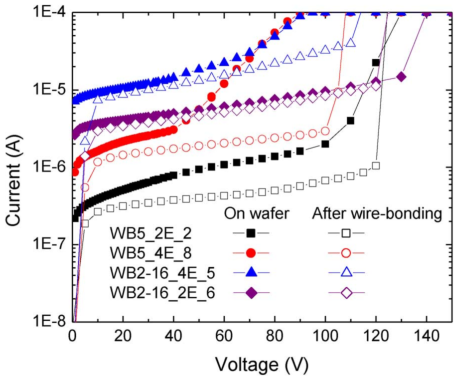
\includegraphics[width=0.45\textwidth]{images/IV_ba.pdf}

  \small    Comparing with the previous measurements done by measuring on the wafer we were able to see that there was an improvement across all the modules after wire-bonding. This is because when the sensors were tested on the wafers only a temporary metal layer was used to connect the columns led to extra leakage current.


 \end{center}
\end{frame}


\begin{frame}{I-V Measurement}
  \begin{center}
    \begin{itemize}
    \item
      On the ROC measured each pixel response for a set bias voltage.
    \item
      For each pixel I fit the IV curve to an S-curve (step function convoluted with a Gaussian).
    \item
      From the slope of the S curve at efficiency of 0.5 we calculate the equivalent noise charge (ENC).
      \begin{equation} ENC = \dfrac{1}{\sqrt{2\pi}}\dfrac{1}{s} \end{equation}
     \end{itemize}
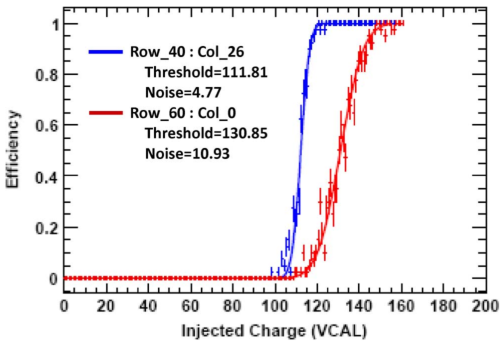
\includegraphics[width=0.45\textwidth]{images/efficiency.pdf}

  \end{center}
\end{frame}

\begin{frame}{Noise}
  \begin{center}
    \begin{itemize}
    \item
      After finding the ENC for each pixel the distribution is fit with a Gaussian.
    \item
      (1 VCAL = 65.5 electrons)
    \end{itemize}
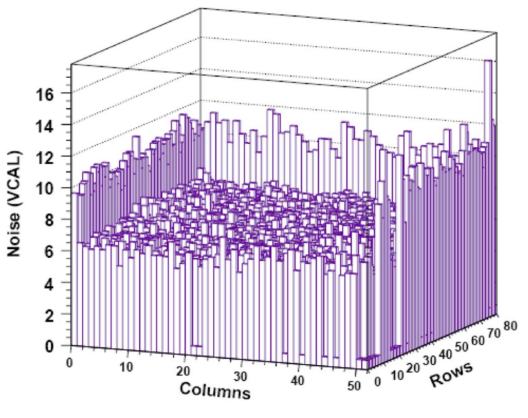
\includegraphics[width=0.45\textwidth]{images/map.pdf}
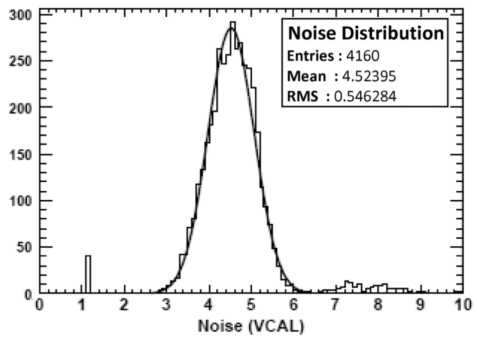
\includegraphics[width=0.45\textwidth]{images/noise.pdf}

  \end{center}
\end{frame}

\begin{frame}{Bias Voltage}
  \begin{center}
    \begin{itemize}
    \item
      Additionally you can calculate these values for varying bias voltages.
    \item
      We found that up till 40 V there is significant improvement but afterward the improvement levels off.
    \end{itemize}
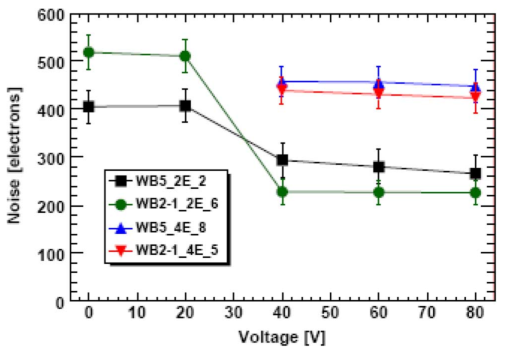
\includegraphics[width=0.65\textwidth]{images/bias.pdf}
%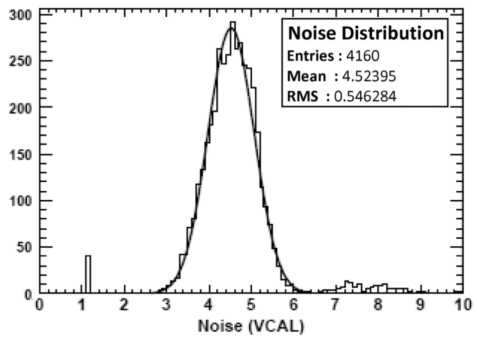
\includegraphics[width=0.45\textwidth]{images/noise.pdf}

  \end{center}
\end{frame}

\begin{frame}{Threshold}
  \begin{center}
    \begin{itemize}
    \item
      The threshold is the voltage where efficiency equals 0.5 on the IV curve.
    \item
      This was measured both with and without trimming.
    \end{itemize}
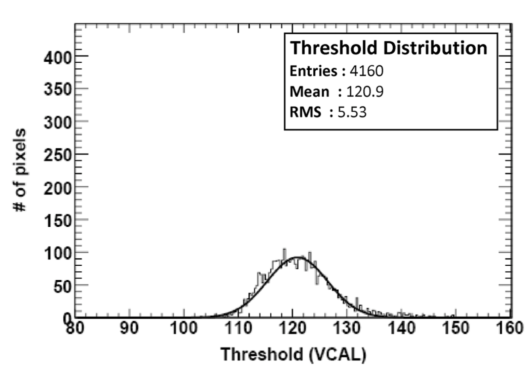
\includegraphics[width=0.45\textwidth]{images/threshold1.pdf}
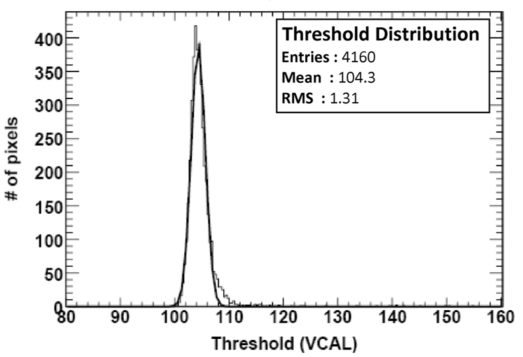
\includegraphics[width=0.45\textwidth]{images/threshold2.pdf}

  \end{center}
\end{frame}

\begin{frame}{Conclusion}
  \begin{center}
    \begin{itemize}
    \item
      The conclusion from my measurements with others in the group was that the signal to threshold (S/T) ratio for these detectors is around 3
    \item
  For the Super LHC you need a S/T ratio of around 4 in midlife and around 3 at the end of life so there needs to be more improvement in the noise for these types of 3D pixels to be acceptable.
    \end{itemize}
  \end{center}
\end{frame}





\end{document}
